\documentclass[aspectratio=169]{beamer}
\usepackage{ferres}
\usepackage{tikz}
\usepackage{algorithm}
\usepackage[noend]{algpseudocode}
\usepackage{capt-of}
\usepackage{subcaption}
%math
\setbeamercolor{alerted text}{fg=red,bg=white}
\input{math_commands.tex}
\newcommand<>\mathalert[1]{{\only#2{\usebeamercolor{alerted text}\color{fg}\setbeamercolor{math text}{fg=fg}}#1}}%

\author{Max Kochurov}
\title{Riemannian Optimization}
\institute{NTechLab}
\begin{document}
\begin{frame}
	\maketitle
\end{frame}
\section{Goals}
\begin{frame}{What is it all for?}
    \begin{enumerate}
        \item We all use optimizers without going deep in math
        \item I have no doubts you can use PyTorch in your research / work
        \item Riemannian Optimization is as easy as SGD, but how to use it properly?
        \item You want some insights about practical usage of Riemannian Optimization
    \end{enumerate}
\end{frame}
\begin{frame}{TL;DR}
\begin{itemize}
    \item Practical implementation with examples is here \url{https://github.com/geoopt/geoopt}
\end{itemize}
\vspace{3em}
\begin{columns}
\begin{column}{0.5\linewidth}

{\Large For some math, stay tuned}
\end{column}

\begin{column}{0.5\linewidth}
\Huge \[\mathcal{T}_p\mathcal{G}\]
\end{column}
\end{columns}
\end{frame}
\section{Motivation}
\subsection{Use Cases}
\begin{frame}{When do we need Riemannian Optimization?}
    \begin{columns}
    \begin{column}{0.5\linewidth}
        \begin{itemize}
            \item<+-> Problem has smooth constraints
            \item<+-> We want to relax the problem
            \item<+-> Accelerate training with adaptive methods
            \item<+-> Perform HMC with constraints
        \end{itemize}
    \end{column}
    \begin{column}{0.5\linewidth}
    \only<1>{
    \center 
    \textbf{Sphere}

    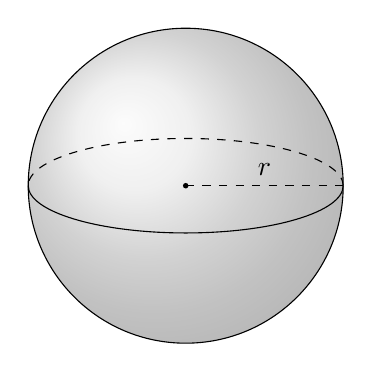
\begin{tikzpicture}
      \shade[ball color = gray!40, opacity = 0.4] (0,0) circle (2cm);
      \draw (0,0) circle (2cm);
      \draw (-2,0) arc (180:360:2 and 0.6);
      \draw[dashed] (2,0) arc (0:180:2 and 0.6);
      \fill[fill=black] (0,0) circle (1pt);
      \draw[dashed] (0,0 ) -- node[above]{$r$} (2,0);
    \end{tikzpicture}
    }
    \only<2>{
        \begin{figure}
            \centering
            \includegraphics[width=\linewidth]{img/birkhoff.png}
            \caption{\url{https://arxiv.org/abs/1904.05814}}
            \label{fig:my_label}
        \end{figure}
        
    }
    \only<3>{
        \begin{figure}
            \centering
            \includegraphics[width=0.8\linewidth]{img/adam_mnist.png}
            \caption{\url{https://arxiv.org/abs/1412.6980}}
            \label{fig:my_label}
        \end{figure}
    }
    \only<4>{
        \begin{figure}
            \centering
            \includegraphics[width=0.8\linewidth]{img/hmc_samples.png}
            \caption{\url{https://arxiv.org/abs/1901.08045}}
            \label{fig:my_label}
        \end{figure}
    }
    \end{column}
    \end{columns}
\end{frame}
\subsection{Alternative Approaches}
\begin{frame}{What else?}
    \begin{columns}
    \begin{column}{0.5\linewidth}
    \begin{itemize}
    \visible<1->{
    \item Reparametrization
    \begin{itemize}
        \item Adaptive terms make sense
        \item HMC is possible
        \item This might be a good idea
    \end{itemize}
    }
    \visible<2>{
    \item Projection
    \begin{itemize}
        \item Adaptive terms do not really make sense
        \item Projection may be hard differentiable (iterative)
    \end{itemize}
    }
    \end{itemize}
    \end{column}
    \begin{column}{0.5\linewidth}
    \begin{tikzpicture}
      \draw (0,0) circle (2cm);
      \fill[fill=black] (0,0) circle (1pt);
      \draw[dashed] (0,0 ) -- node[above]{$v/\|v\|$} (2,0);
      \draw[dashed] (2,0 ) -- node[right,above]{$v$} (3,0);
      \fill[fill=black] (2,0) circle (1pt);
      \fill[fill=black] (3,0) circle (1pt);
    \end{tikzpicture}
    \end{column}
    \end{columns}
\end{frame}
\section{SGD Review}
\begin{frame}{Riemannian AMS grad}
\vspace{-0.5em}
    \begin{figure}
\begin{subfigure}{.45\textwidth}
\centering
\begin{algorithmic}
    \Require $x_1\in\mathcal{X}$, $\lbrace\alpha_t\rbrace_{t=1}^T$, $\lbrace\beta_{1t}\rbrace_{t=1}^T$, $\beta_2$\\
    Set $m_0=0$, $v_0=0$ and $\hat{v}_0=0$
    \For{$t=1$ to $T$} (for all $1\leq i\leq n$)
    \State $\alert<2,7>{g_t=\mathrm{grad} f_t(x_t)}$
    \State $\alert<3,8>{m_t^i=\beta_{1t}m_{t-1}^i+(1-\beta_{1t}) g_t^i}$
    \State $\alert<4,9>{v_t^i=\beta_2 v_{t-1}^i + (1-\beta_2)(g_t^{i})^2}$
    \State $\alert<4,9>{\hat{v}_t^i=\max\{\hat{v}_{t-1}^i,v_t^i\}}$
    \State $\alert<5,10>{x_{t+1}^i=x_{t}^i-\alpha_t m_t^i/\sqrt{\hat{v}_t^i}}$\\
    \visible<8->{\alert<8>{\Comment{no vector transport}}\\}
    \textbf{end\ for}
    \EndFor\\
\end{algorithmic}
    \caption{\textsc{Amsgrad} in $\mathbb{R}^n$.}\label{alg:alg-2}
\end{subfigure}
\hfill
\visible<6->{
\begin{subfigure}{.45\textwidth}
\centering
\begin{algorithmic}
    \Require $x_1\in\mathcal{X}$, $\lbrace\alpha_t\rbrace_{t=1}^T$, $\lbrace\beta_{1t}\rbrace_{t=1}^T$, $\beta_2$\\
    Set $m_0=0$, $\tau_0=0$, $v_0=0$ and $\hat{v}_0=0$
    \For{$t=1$ to $T$} (for all $1\leq i\leq n$)
    \State $\alert<7>{g_t=\mathrm{rgrad} f_t(x_t)}$ 
    \State $\alert<8>{m_t^i=\beta_{1t}\tau_{t-1}^i+(1-\beta_{1t}) g_t^i}$
    \State $\alert<9>{v_t^i=\beta_2 v_{t-1}^i + (1-\beta_2)\Vert g_t^{i}\Vert_{x_t^i}^2}$
    \State $\alert<9>{\hat{v}_t^i=\max\{\hat{v}_{t-1}^i,v_t^i\}}$
    \State $\alert<10>{x_{t+1}^i=\exp^i_{x_{t}^i}(-\alpha_t m_t^i/\sqrt{\hat{v}_t^i})}$
    \State $\alert<8>{\tau_t^i=P^i_{x_t^i\to x_{t+1}^i}(m_t^i)}$\\
    \textbf{end\ for}
    \EndFor\\
\end{algorithmic}
    \caption{\textsc{Ramsgrad} in $\mathcal{M}_1\times\cdots\times\mathcal{M}_n$.}
    \label{alg:alg-1}
\end{subfigure}
}
\end{figure}
Comment: %
\only<2>{we need gradients, in \texttt{pytorch} it would be \texttt{loss.backward()}}%
\only<3>{keep track of momentum at each iteration}%
\only<4>{update adaptive terms using second moments of the gradient}%
\only<5>{sure we make final gradient step}%
\only<6>{what is the difference for Riemannian case?}%
\only<7>{gradient stays \textit{almost} the same, \texttt{loss.backward()} and correction}%
\only<8>{momentum update requires new operation, \textit{``vector transport''} $P^i_{x_t^i\to x_{t+1}^i}$}%
\only<9>{adaptive term depends on the current point via$\Vert g_t^{i}\Vert_{x_t^i}^2$}%
\only<10>{there is no addition between vectors and points}
\end{frame}
\begin{frame}{Blank Spots}
\begin{columns}
\begin{column}{0.5\linewidth}
\begin{enumerate}
    \item<+-> How to properly work with gradients?
    \item<+-> Why some computations depend on the point of application?
    \item<+-> How to work with momentums?
    \item<+-> How to make the final update?
\end{enumerate}
\visible<+->{
    \begin{block}{}
    We will review all this in the next section
    \end{block}
}
\end{column}
\begin{column}{0.5\linewidth}
\begin{figure}
    \centering
    \includegraphics[width=0.8\linewidth]{img/thinkingface.png}
\end{figure}
\end{column}
\end{columns}
\end{frame}
\section{Differential Geometry}
\subsection{Manifold}
\begin{frame}{What is Manifold?}
\begin{columns}
\begin{column}{0.5\linewidth}
The best example I know is actually Sphere! 
\visible<2->{
\begin{block}{}
A curious researcher (a kid) may ask questions
\end{block}
\begin{enumerate}
    \item<2-> Is it really a sphere or anything else?
    \item<3-> What makes a sphere be a sphere?
    \item<4> How to represent a point on earth?
\end{enumerate}
}
\end{column}
\begin{column}{0.5\linewidth}
\only<1>{
\begin{figure}
    \centering
    \includegraphics[width=0.8\linewidth]{img/earth.jpg}
    \caption*{Looks like a sphere}
\end{figure}
}%
\only<2>{
\begin{figure}
    \centering
    \includegraphics[width=\linewidth]{img/flatearth.jpg}
    \caption*{Or simulation?}
\end{figure}
}%
\only<3>{
\begin{figure}
\centering
\begin{subfigure}{0.5\linewidth}
\centering
    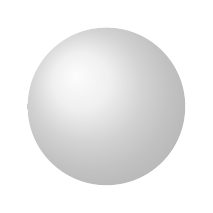
\begin{tikzpicture}
      \shade[ball color = gray!40, opacity = 0.4] (0,0) circle (1cm);
    \end{tikzpicture}
    \caption*{sphere}
\end{subfigure}%
\begin{subfigure}{0.5\linewidth}
\centering
\includegraphics[width=\linewidth]{img/potato.jpeg}
\caption*{also a sphere}
\end{subfigure}
\caption*{Topology joke}
\end{figure}
}%
\only<4>{
\centering
\includegraphics[height=2cm]{img/map1.jpg}
\includegraphics[height=2cm]{img/map2.jpg}\\
\includegraphics[height=2cm]{img/map3.png}
\includegraphics[height=2cm]{img/map4.jpg}\\
}
\end{column}
\end{columns}
\end{frame}
\begin{frame}{Earth is Math}
\begin{columns}
\begin{column}{0.5\linewidth}
\begin{itemize}
    \item ``Sphereness'' is an intrinsic property, we can touch it, but how?
\end{itemize}
\begin{block}{enough?}
\begin{equation*}
    \left\{\|x\| = 1\::\: x \in \sR \right\} 
\end{equation*}
\end{block}
\pause
\begin{alertblock}{}
no
\end{alertblock}
\end{column}
\begin{column}{0.5\linewidth}
\begin{figure}
    \centering
    \includegraphics[width=0.8\linewidth]{img/sputnik.jpg}
    \caption*{It's all nature, and we can observe it with experience}
\end{figure}
\end{column}
\end{columns}
\end{frame}
\begin{frame}{Earth is more Math}
\begin{columns}
\begin{column}{0.5\linewidth}
We can represent sphere in many ways:
\begin{block}{Constraints}
\begin{equation*}
    \left\{\|x\| = 1\::\: x \in \sR \right\} 
\end{equation*}
\end{block}
\begin{block}{Parametrization}
\begin{equation*}
    \left\{\theta\in (0, \pi), \phi\in (0, \pi)\right\} 
\end{equation*}
\end{block}

\end{column}
\begin{column}{0.5\linewidth}
\begin{figure}
\centering
    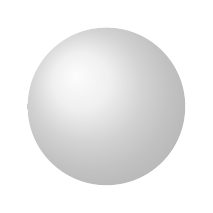
\begin{tikzpicture}
      \shade[ball color = gray!40, opacity = 0.4] (0,0) circle (1cm);
    \end{tikzpicture}
\end{figure}%
\end{column}
\end{columns}
\end{frame}
\subsection{Tangent Space}
\subsection{Curves}
\subsection{Inner Product}
\subsection{Vector Transport}
\section{Filling Blank Spots}
\subsection{Computing Gradient}
\subsection{Computing Adaptive Term}
\subsection{Updating Momentum}
\section{Practical Implementation}
\end{document}
